\serie{Développer}


\begin{exercice}[]
Développe puis réduis les expressions :
\begin{colenumerate}{2}
\item $A = 3 \times (x + 2)$
\item $B = 7 \times (x - 6)$
\item $C = 1 \times (x + 5)$
\item $D = 4 \times (5 - x)$
\item $E = 1,6(x - 0,5)$
\item $F = 4(x + 1)$
\item $G = 7(3x - 8)$
\item $H = 6(2x + 9)$
\end{colenumerate}
\end{exercice}

\begin{exercice}[]
Développe puis réduis les expressions :
\begin{colenumerate}{2}
\item $A = x(x + 2)$
\item $B = x(x - 6)$
\item $C = 3x(x + 5)$
\item $D = 5x(x - 1)$
\item $E = 6x(2 + 9x)$
\item $F = x(x^2 - 4)$
\end{colenumerate}
\end{exercice}

\begin{exercice}[]
Développe les expressions suivantes :
\begin{colenumerate}{2}
\item $A = 3(x + 6)$
\item $B = 5(6 -y)$
\item $C = -7(2z -3)$
\item $D = -8(-5 -3y)$
\item $E = 6(4x -9)$
\item $F = -12(-5 + 3z)$
\end{colenumerate}
\end{exercice}

\begin{exercice}[]
Développe les expressions suivantes :
\begin{colenumerate}{2}
\item $A = (-3 + y) \times 9$
\item $B = -6(2x -7)$
\item $C = (3t + 2) \times 8$
\item $D = -8(9 -7x)$
\item $E = -8z(4 -3z)$
\item $F = 3y(-4 + 6y)$
\end{colenumerate}
\end{exercice}

\begin{exercice}[]
Développe les expressions suivantes :
\begin{colenumerate}{2}
\item $A = x(x + 4)$
\item $B = 7y(2 - 9y)$
\item $C = -2y(5 -y)$
\item $D = (9 -3t) \times 4t$
\end{colenumerate}
\end{exercice}

\begin{exercice}[]
Développe et réduis les expressions :
\begin{colenumerate}{2}
\item $A = 11 + 2(x -6)$
\item $B = -3(2y -4) -2y$
\item $C = 7 -4(8 -2a) + a$
\item $D = -15 -9(-5 + 3b)$
\item $E = -5(6 -3z) -9 + z$
\item $F = 12x -4(6 -3x)$
\end{colenumerate}
\end{exercice}

\begin{exercice}[]
Développe et réduis les expressions :
\begin{colenumerate}{1}
\item $A = 3x -5 + 5(2x -2)$
\item $B = 4y -6(3 -2y) + 4(y -1)$
\item $C = 5t^2 + 3(2t -3) -2t(t -5)$
\end{colenumerate}
\end{exercice}



\serie{Double distributivité}





\begin{exercice}[]
Développe et réduis les expressions :
\begin{colenumerate}{2}
\item $A = (x + 4)(x + 3)$
\item $B = (y + 3)(2y + 8)$
\item $C = (3z + 4)(5 -6z)$
\item $D = (-7t + 8)(3 -5t)$
\end{colenumerate}
\end{exercice}

\begin{exercice}[]
Développe et réduis les expressions :
\begin{colenumerate}{2}
\item $A = (7 -3x)(9x -3)$
\item $B = (-2 -3y)(4 -8y)$
\item $C = (4a + 6)(-3 -5a)$
\item $D = (5z -7)(8z + 2)$
\end{colenumerate}
\end{exercice}

\begin{exercice}[]
Développe et réduis les expressions :
\begin{colenumerate}{2}
\item $A = (a + 1)^2$
\item $B = (5x + 2)^2$
\item $C = (3y -4)^2$
\item $D = (4 -x)^2$
\end{colenumerate}
\end{exercice}

\begin{exercice}[]
Développe et réduis les expressions :
\begin{colenumerate}{2}
\item $A = 3(x + 1)(x -5)$
\item $B = 2(-3 -t)(t -7)$
\item $C = -(y + 5)(3y -6)$
\item $D = x(2x -5)(2 -x)$
\end{colenumerate}
\end{exercice}

\begin{exercice}[]
On considère les expressions :

\[A = (x + 2)(x -3) + (x -3) \quad \text{et} \quad B = (2x -3)^2 \]

\begin{colenumerate}{1} 
\item Développer et réduire les deux expressions.
\item Calculer $A$ pour $x = 3$.
\item Calculer $B$ pour $x = 1,5$.
\end{colenumerate} 
 
\end{exercice}

\begin{exercice}[]
On considère le rectangle ci-dessous. Exprime en fonction de $x$ :

\begin{center}
    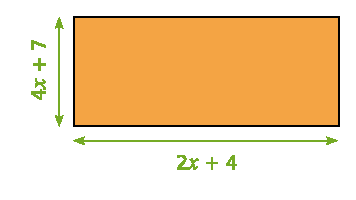
\includegraphics[width=.7\linewidth]{DiEe01}
\end{center}

\begin{colenumerate}{1} 
\item son périmètre sous la forme d'une expression réduite ;
\item son aire sous la forme d'une expression factorisée ;
\item son aire sous la forme d'une expression développée et réduite.
\end{colenumerate} 
 
\end{exercice}

\begin{exercice}[]
Parmi les expressions suivantes, retrouve celles qui sont égales et justifie ta réponse :
\begin{colenumerate}{2}
\item $A = 16 -4x2$
\item $B = (4 -2x)^2$
\item $C = (4 -2x)(4 + 2x)$
\item $D = 4x2 -16x + 16$
\end{colenumerate}
\end{exercice}
